\documentclass[xcolor=dvipsnames,14pt]{beamer}
\beamertemplatenavigationsymbolsempty%Turn off the navbar
\usepackage{geometry}
\usepackage{minted}
\usepackage{graphicx}
\usepackage{codehilite}
\usepackage{macros}


\newcommand{\punt}[1]{}

\begin{document}
\title{SuperMalloc}
\subtitle{A fast HTM-friendly memory allocator with a small footprint}

\author{Bradley C. Kuszmaul}
\date{CSAIL PL Offsite, May  15, 2015}
\frame{\titlepage}

\begin{frame}[fragile]
\frametitle{Malloc and Free}
\begin{minted}[mathescape]{c}
void* malloc(size_t s);
\end{minted}

Effect: Allocate and return a pointer to a block of memory containing at least "s" bytes.

\begin{minted}{c}
void free(void *p);
\end{minted}

Effect: "p" is a pointer to a block of memory returned by "malloc()".  Deallocate the block.
\end{frame}

\begin{frame}[fragile]
\frametitle{Aligned Allocation}

\begin{minted}[mathescape]{c}
void* memalign(size_t alignment, size_t s);
\end{minted}


Effect: Allocate and return a pointer to a block of memory containing at least "s" bytes.  
The returned pointer shall be a multiple of "alignment".  That is,
\begin{center}
"0 == (size_t)(memalign(a, s)) % a}"
\end{center}

Requires: "a" is a power of two.
\end{frame}

\begin{frame}
\frametitle{DLmalloc}

Linux libc employs Doug Lea's malloc, which dates from 1987.

\begin{itemize}
\item DLmalloc suffers high space overhead (an 8-byte boundary tag on every object, and poor space reclamation).
\item DLmalloc is slow (especially on multithreaded code, where it uses a monolithic lock).
\end{itemize}

To address these problems, allocators such as Hoard, TCmalloc, JEmalloc have appeared.

\end{frame}

\begin{frame}[fragile]
\frametitle{Modern Allocators Employ Thread Caches}

\begin{minted}[mathescape]{c}
__thread LinkedList *cache[N_SIZE_CLASSES];

void *alloc(size_t s) {
  int size_class = size_2_class(s);
  void *ret = cache[size_class];
  if (ret != NULL) {
    cache[size_class] = ret->next;
    return ret;
  }
  ...
\end{minted}

A call to the allocator requires no locking if it can be satisfied by the cache .
\end{frame}

\begin{frame}[fragile]
\frametitle{Thread Caches are Really Fast}

\begin{minted}[mathescape]{c}
while (1) {
  free(malloc(8));
}
\end{minted}

\begin{itemize}
\item Used by the original Cilk allocator [BlumofeLe94], the early STL allocator [SGI97], PTmalloc [Gloger06], LKmalloc[LarsonKr98], and TCmalloc [Google13].
\item No locks, so it's really fast.
\item Must take a little care to avoid false cache-line sharing.
\item What goes wrong?
\end{itemize}
\end{frame}

\begin{frame}[fragile]
\frametitle{The Malloc-test Benchmark}

\begin{itemize}
\item Benchmark due to Lever, Boreham, and Eder.
\textit{malloc() Performance in a Multithreaded Linux
  Environment}, USENIX 2000.

\item $k$ allocator threads, $k$ deallocator threads.

\item Each allocator thread calls "malloc()" as fast as it can and hands the object to a deallocator thread, which calls "free()" as fast as it can.

\item It's a tough (maybe the toughest) benchmark, because per-thread caches become unbalanced.

\item The code is racy, and produces noisy data.  I sped it up by a factor of two, and de-noised it.
\end{itemize}

\end{frame}

\begin{frame}[fragile]
\frametitle{Allocators that Also Focused on Space}

\begin{itemize}
\item Hoard [BergerMcBl00] Provided the first space bound for allocators
with thread caches.
\item TBBMalloc [KukanovVo07] adopted a later Cilk allocator (but still has a footprint problem sometimes).
\item JEmalloc [Evans06] seems to be the best incumbent.
\end{itemize}


\end{frame}

\begin{frame}
\frametitle{Malloc-test on a 4-core Haswell (with Hyperthreading)}

% GNUPLOT: LaTeX picture with Postscript
\begingroup
  \fontfamily{ptm}%
  \selectfont
  \makeatletter
  \providecommand\color[2][]{%
    \GenericError{(gnuplot) \space\space\space\@spaces}{%
      Package color not loaded in conjunction with
      terminal option `colourtext'%
    }{See the gnuplot documentation for explanation.%
    }{Either use 'blacktext' in gnuplot or load the package
      color.sty in LaTeX.}%
    \renewcommand\color[2][]{}%
  }%
  \providecommand\includegraphics[2][]{%
    \GenericError{(gnuplot) \space\space\space\@spaces}{%
      Package graphicx or graphics not loaded%
    }{See the gnuplot documentation for explanation.%
    }{The gnuplot epslatex terminal needs graphicx.sty or graphics.sty.}%
    \renewcommand\includegraphics[2][]{}%
  }%
  \providecommand\rotatebox[2]{#2}%
  \@ifundefined{ifGPcolor}{%
    \newif\ifGPcolor
    \GPcolortrue
  }{}%
  \@ifundefined{ifGPblacktext}{%
    \newif\ifGPblacktext
    \GPblacktextfalse
  }{}%
  % define a \g@addto@macro without @ in the name:
  \let\gplgaddtomacro\g@addto@macro
  % define empty templates for all commands taking text:
  \gdef\gplbacktext{}%
  \gdef\gplfronttext{}%
  \makeatother
  \ifGPblacktext
    % no textcolor at all
    \def\colorrgb#1{}%
    \def\colorgray#1{}%
  \else
    % gray or color?
    \ifGPcolor
      \def\colorrgb#1{\color[rgb]{#1}}%
      \def\colorgray#1{\color[gray]{#1}}%
      \expandafter\def\csname LTw\endcsname{\color{white}}%
      \expandafter\def\csname LTb\endcsname{\color{black}}%
      \expandafter\def\csname LTa\endcsname{\color{black}}%
      \expandafter\def\csname LT0\endcsname{\color[rgb]{1,0,0}}%
      \expandafter\def\csname LT1\endcsname{\color[rgb]{0,1,0}}%
      \expandafter\def\csname LT2\endcsname{\color[rgb]{0,0,1}}%
      \expandafter\def\csname LT3\endcsname{\color[rgb]{1,0,1}}%
      \expandafter\def\csname LT4\endcsname{\color[rgb]{0,1,1}}%
      \expandafter\def\csname LT5\endcsname{\color[rgb]{1,1,0}}%
      \expandafter\def\csname LT6\endcsname{\color[rgb]{0,0,0}}%
      \expandafter\def\csname LT7\endcsname{\color[rgb]{1,0.3,0}}%
      \expandafter\def\csname LT8\endcsname{\color[rgb]{0.5,0.5,0.5}}%
    \else
      % gray
      \def\colorrgb#1{\color{black}}%
      \def\colorgray#1{\color[gray]{#1}}%
      \expandafter\def\csname LTw\endcsname{\color{white}}%
      \expandafter\def\csname LTb\endcsname{\color{black}}%
      \expandafter\def\csname LTa\endcsname{\color{black}}%
      \expandafter\def\csname LT0\endcsname{\color{black}}%
      \expandafter\def\csname LT1\endcsname{\color{black}}%
      \expandafter\def\csname LT2\endcsname{\color{black}}%
      \expandafter\def\csname LT3\endcsname{\color{black}}%
      \expandafter\def\csname LT4\endcsname{\color{black}}%
      \expandafter\def\csname LT5\endcsname{\color{black}}%
      \expandafter\def\csname LT6\endcsname{\color{black}}%
      \expandafter\def\csname LT7\endcsname{\color{black}}%
      \expandafter\def\csname LT8\endcsname{\color{black}}%
    \fi
  \fi
  \setlength{\unitlength}{0.0500bp}%
  \begin{picture}(4320.00,2720.00)%
    \gplgaddtomacro\gplbacktext{%
      \csname LTb\endcsname%
      \put(538,558){\makebox(0,0)[r]{\strut{}\footnotesize 0}}%
      \csname LTb\endcsname%
      \put(538,1156){\makebox(0,0)[r]{\strut{}\footnotesize $50$M}}%
      \csname LTb\endcsname%
      \put(538,1694){\makebox(0,0)[r]{\strut{}\footnotesize $95$M}}%
      \csname LTb\endcsname%
      \put(809,298){\makebox(0,0){\strut{} 1}}%
      \csname LTb\endcsname%
      \put(1283,298){\makebox(0,0){\strut{} 2}}%
      \csname LTb\endcsname%
      \put(1758,298){\makebox(0,0){\strut{} 3}}%
      \csname LTb\endcsname%
      \put(2232,298){\makebox(0,0){\strut{} 4}}%
      \csname LTb\endcsname%
      \put(2706,298){\makebox(0,0){\strut{} 5}}%
      \csname LTb\endcsname%
      \put(3181,298){\makebox(0,0){\strut{} 6}}%
      \csname LTb\endcsname%
      \put(3655,298){\makebox(0,0){\strut{} 7}}%
      \csname LTb\endcsname%
      \put(4129,298){\makebox(0,0){\strut{} 8}}%
      \csname LTb\endcsname%
      \put(88,1359){\rotatebox{-270}{\makebox(0,0){\small \texttt{malloc()}'s per second}}}%
      \csname LTb\endcsname%
      \put(2516,19){\makebox(0,0){\small Producer threads}}%
      \put(2516,2440){\makebox(0,0){\strut{}\small 4-Core (8 hardware threads) 3.4GHz Haswell}}%
      \csname LTb\endcsname%
      \put(2516,2067){\makebox(0,0){\strut{}}}%
      \colorrgb{0.00,0.39,0.00}%
      \put(2090,1515){\makebox(0,0)[r]{\strut{}\footnotesize SuperMalloc}}%
      \colorrgb{0.63,0.00,0.00}%
      \put(2706,644){\makebox(0,0)[r]{\strut{}\footnotesize dlmalloc}}%
      \colorrgb{0.00,0.00,0.63}%
      \put(4082,678){\makebox(0,0)[r]{\strut{}\footnotesize Hoard}}%
      \colorrgb{0.63,0.00,0.63}%
      \put(4129,989){\makebox(0,0)[r]{\strut{}\footnotesize jemalloc}}%
    }%
    \gplgaddtomacro\gplfronttext{%
    }%
    \gplbacktext
    \put(0,0){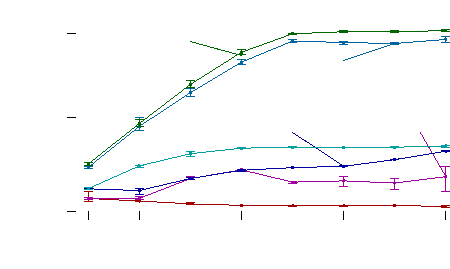
\includegraphics{new-malloc-test-1K-lutestring-aggregated}}%
    \gplfronttext
  \end{picture}%
\endgroup

\end{frame}
\begin{frame}
\frametitle{Malloc-test on a 16-core Haswell (with Hyperthreading)}

% GNUPLOT: LaTeX picture with Postscript
\begingroup
  \fontfamily{ptm}%
  \selectfont
  \makeatletter
  \providecommand\color[2][]{%
    \GenericError{(gnuplot) \space\space\space\@spaces}{%
      Package color not loaded in conjunction with
      terminal option `colourtext'%
    }{See the gnuplot documentation for explanation.%
    }{Either use 'blacktext' in gnuplot or load the package
      color.sty in LaTeX.}%
    \renewcommand\color[2][]{}%
  }%
  \providecommand\includegraphics[2][]{%
    \GenericError{(gnuplot) \space\space\space\@spaces}{%
      Package graphicx or graphics not loaded%
    }{See the gnuplot documentation for explanation.%
    }{The gnuplot epslatex terminal needs graphicx.sty or graphics.sty.}%
    \renewcommand\includegraphics[2][]{}%
  }%
  \providecommand\rotatebox[2]{#2}%
  \@ifundefined{ifGPcolor}{%
    \newif\ifGPcolor
    \GPcolortrue
  }{}%
  \@ifundefined{ifGPblacktext}{%
    \newif\ifGPblacktext
    \GPblacktextfalse
  }{}%
  % define a \g@addto@macro without @ in the name:
  \let\gplgaddtomacro\g@addto@macro
  % define empty templates for all commands taking text:
  \gdef\gplbacktext{}%
  \gdef\gplfronttext{}%
  \makeatother
  \ifGPblacktext
    % no textcolor at all
    \def\colorrgb#1{}%
    \def\colorgray#1{}%
  \else
    % gray or color?
    \ifGPcolor
      \def\colorrgb#1{\color[rgb]{#1}}%
      \def\colorgray#1{\color[gray]{#1}}%
      \expandafter\def\csname LTw\endcsname{\color{white}}%
      \expandafter\def\csname LTb\endcsname{\color{black}}%
      \expandafter\def\csname LTa\endcsname{\color{black}}%
      \expandafter\def\csname LT0\endcsname{\color[rgb]{1,0,0}}%
      \expandafter\def\csname LT1\endcsname{\color[rgb]{0,1,0}}%
      \expandafter\def\csname LT2\endcsname{\color[rgb]{0,0,1}}%
      \expandafter\def\csname LT3\endcsname{\color[rgb]{1,0,1}}%
      \expandafter\def\csname LT4\endcsname{\color[rgb]{0,1,1}}%
      \expandafter\def\csname LT5\endcsname{\color[rgb]{1,1,0}}%
      \expandafter\def\csname LT6\endcsname{\color[rgb]{0,0,0}}%
      \expandafter\def\csname LT7\endcsname{\color[rgb]{1,0.3,0}}%
      \expandafter\def\csname LT8\endcsname{\color[rgb]{0.5,0.5,0.5}}%
    \else
      % gray
      \def\colorrgb#1{\color{black}}%
      \def\colorgray#1{\color[gray]{#1}}%
      \expandafter\def\csname LTw\endcsname{\color{white}}%
      \expandafter\def\csname LTb\endcsname{\color{black}}%
      \expandafter\def\csname LTa\endcsname{\color{black}}%
      \expandafter\def\csname LT0\endcsname{\color{black}}%
      \expandafter\def\csname LT1\endcsname{\color{black}}%
      \expandafter\def\csname LT2\endcsname{\color{black}}%
      \expandafter\def\csname LT3\endcsname{\color{black}}%
      \expandafter\def\csname LT4\endcsname{\color{black}}%
      \expandafter\def\csname LT5\endcsname{\color{black}}%
      \expandafter\def\csname LT6\endcsname{\color{black}}%
      \expandafter\def\csname LT7\endcsname{\color{black}}%
      \expandafter\def\csname LT8\endcsname{\color{black}}%
    \fi
  \fi
  \setlength{\unitlength}{0.0500bp}%
  \begin{picture}(4320.00,2580.00)%
    \gplgaddtomacro\gplbacktext{%
      \csname LTb\endcsname%
      \put(538,558){\makebox(0,0)[r]{\strut{}\footnotesize 0}}%
      \csname LTb\endcsname%
      \put(538,1236){\makebox(0,0)[r]{\strut{}\footnotesize$50$M}}%
      \csname LTb\endcsname%
      \put(538,1914){\makebox(0,0)[r]{\strut{}\footnotesize$100$M}}%
      \csname LTb\endcsname%
      \put(538,2375){\makebox(0,0)[r]{\strut{}\footnotesize $134$M}}%
      \csname LTb\endcsname%
      \put(827,298){\makebox(0,0){\strut{} 1}}%
      \csname LTb\endcsname%
      \put(1615,298){\makebox(0,0){\strut{} 8}}%
      \csname LTb\endcsname%
      \put(2517,298){\makebox(0,0){\strut{} 16}}%
      \csname LTb\endcsname%
      \put(3418,298){\makebox(0,0){\strut{} 24}}%
      \csname LTb\endcsname%
      \put(4319,298){\makebox(0,0){\strut{} 32}}%
      \csname LTb\endcsname%
      \put(37,1466){\rotatebox{-270}{\makebox(0,0){\small \texttt{malloc()}'s per second}}}%
      \csname LTb\endcsname%
      \put(2516,19){\makebox(0,0){\small Producer threads}}%
      \put(2516,2282){\makebox(0,0){\strut{}}}%
      \csname LTb\endcsname%
      \put(2516,2281){\makebox(0,0){\strut{}}}%
      \colorrgb{0.00,0.39,0.00}%
      \put(2404,2185){\makebox(0,0)[r]{\strut{}\footnotesize SuperMalloc}}%
      \colorrgb{0.63,0.00,0.00}%
      \put(2742,639){\makebox(0,0)[r]{\strut{}\footnotesize dlmalloc}}%
      \colorrgb{0.63,0.00,0.63}%
      \put(4319,944){\makebox(0,0)[r]{\strut{}\footnotesize Hoard}}%
      \colorrgb{0.00,0.00,0.63}%
      \put(4094,1128){\makebox(0,0)[r]{\strut{}\footnotesize jemalloc}}%
    }%
    \gplgaddtomacro\gplfronttext{%
    }%
    \gplbacktext
    \put(0,0){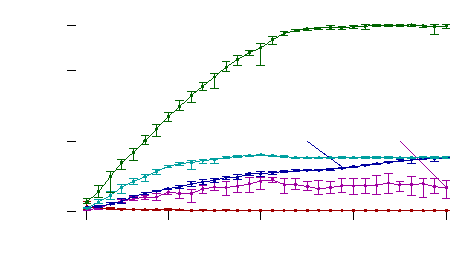
\includegraphics{new-malloc-test-1K-tempo-aggregated}}%
    \gplfronttext
  \end{picture}%
\endgroup

\end{frame}

\begin{frame}
\frametitle{SuperMalloc Strategies}

\begin{itemize}
\item Can waste some virtual space: it's $2^{48}$ bytes.
\item Don't waste RSS ($2^{40}$ bytes on big machines).
\item Contention costs dearly, not locking.  Use a per-CPU cache.
\item Make per-CPU cache smaller than L3 cache, since the application
  has cache misses anyway.
\item Thread cache should be just big enough to reduce locking overhead.  (About 10 objects.)
\item Use Hardware transactional memory (HTM).
\item HTM likes simple data structures.  Use a big array instead of a red-black tree.
\item Object sizes should be a prime number of cache lines to avoid associativity conflicts.
\end{itemize}

I'll talk briefly about locking.
\end{frame}

\begin{frame}[fragile]
\frametitle{Costs of Locking vs. Cache Contention}

I measured the cost of updating a variable in a multithreaded code.

\begin{tabular}{rr}
                                                  global variable &    193.6ns \\
            per cpu (always call "sched_getcpu()"  &     30.2ns \\
per cpu (cache getcpu, refresh/32) &     17.0ns \\
                                                      per thread &      3.1ns \\
                                                  local in stack &      3.1ns \\
\end{tabular}

How to use this:  Make a per-thrad cache that's just big enough to amortize the locking instruction, and then use a per-CPU cache.
\end{frame}

\begin{frame}
\frametitle{SuperMalloc is Available}

From {\small \url{https://github.mit.edu/SuperTech/SuperMalloc}},

or downstream at {\small \url{https://github.com/kuszmaul/SuperMalloc}}.

Dual licensed under MIT Expat and GPLv3.
\end{frame}

\end{document}
\punt{
\begin{frame}
\frametitle{Doug Lea's Goals For Malloc}

\begin{columns}
\hspace*{-.3cm}
\begin{column}{1.15 \textwidth}
\begin{description}[Error Detection:]
\item[Compatibility:] POSIX API.
\item[Portability:] SuperMalloc now works only on x86-64/Linux (and likes Haswell).
\item[Space:] SuperMalloc wins.
\item[Time:] SuperMalloc wins on average time.  Difficult to measure worst case.
\item[Tunability:] I hate tunability.
\item[Locality:] Objects allocated at the same time should be near each other.  Nobody seems to care.
\item[Error Detection:] SuperMalloc performs little checking.
\item[Anomalies:] I'm hopeful.
\end{description}
\end{column}
\end{columns}
\end{frame}
}


\begin{frame}
\frametitle{Malloc-test on Some Existing Allocators}
\hspace*{-.7cm}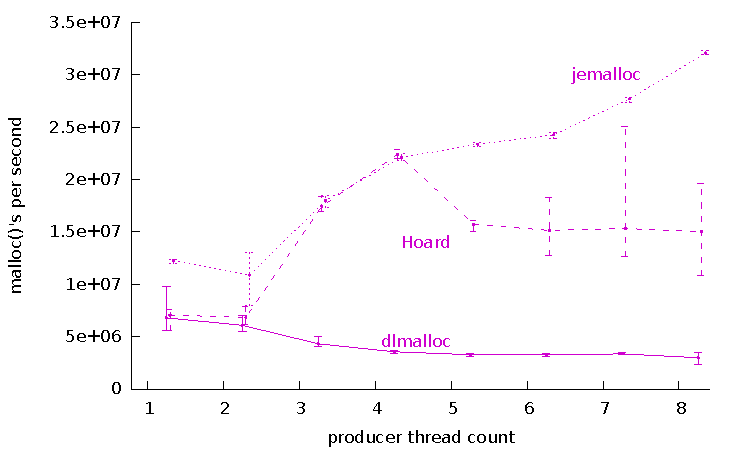
\includegraphics{new-malloc-test-1K-aggregated-oldallocators.pdfn}
\end{frame}

\begin{frame}
\frametitle{Worst Case Time is Bad}

My motivation: jemalloc seems to be the best allocator right now.  It
is much faster than dlmalloc, and its memory footprint is half for
long-lived processes (such as database servers).

\vfill
However: In jemalloc, once per day \mintinline{c}{free()} takes 3 seconds.

\vfill
I suspect lock-holder preemption, but it's tough to observe.
\end{frame}

\begin{frame}
\frametitle{DLmalloc Employs Bins}
A bin is a doubly linked list of free objects that are all close to the same size.

\vfill

For example, dlmalloc employs 32 ``small'' bins of size 8, 16, 24, 32,
\ldots, 256 bytes respectively.  If you allocate 12 bytes, you get a 16-byte object.

\end{frame}

\begin{frame}
\frametitle{DLmalloc Employs Boundary Tags}

Put the size before every object and after every free object.  The
tag also indicates whether the object and previous object are free or in use.

\begin{center}
\begin{tabular}{l|l|}
                                                    \hline
an allocated chunk & size (this in use)                \\ \cline{2-2}
                   & $\ldots$ user data $\ldots$ \\ \hline
a free chunk       & size (this free, prev in use)     \\ \cline{2-2}
                   & pointer to next chunk in bin \\ \cline{2-2}
                   & pointer to prev chunk in bin \\ \cline{2-2}
                   & $\ldots$ unused space $\ldots$ \\ \cline{2-2}
                   & size                        \\ \hline
an allocated chunk & size (this in use, prev free)    \\ \cline{2-2}
                   & $\ldots$ user data $\ldots$ \\ \hline
\end{tabular}
\end{center}
\end{frame}

\begin{frame}
\frametitle{DLmalloc malloc()}

\begin{itemize}
\item Find any object in the smallest nonempty bin that is big enough.

\item If none available, get  more memory from operating system.

\item Historically: Earlier versions of dlmalloc implemented first-fit within each bin.

They kept the bins sorted (but maintaining a heap in each bin would
have been enough).

\item Now it's more complex.

\item Operation complexity is $O(\mbox{\mintinline{c}{sizeof(size_t)}})$.
\end{itemize}
\end{frame}
  
\begin{frame}
\frametitle{DLmalloc free()}

\begin{enumerate}
\item Remove adjacent free blocks (if any) from their bins.
\item Coalesce adjacent free blocks.
\item Put the resulting free block in the right bin.
\end{enumerate}
\end{frame}

\begin{frame}
\frametitle{DLmalloc is simple, but slow}

\begin{tabular}{rrr}
         & lines of code & malloc\_test speed \\
dlmalloc &    6,281 &  3.0M/s \\
hoard    &   16,948 &  5.2M/s \\
jemalloc    & 22,230 & \\
SuperMalloc & 3,571 & 15.1M/s \\
\end{tabular}

\vfill

malloc\_test allocates objects in two threads and frees them in
two others.  ``Speed'' is mallocs per second.

\end{frame}

\begin{frame}
\frametitle{DLmalloc suffers an 8-byte/object overhead}

Since each object is preceeded by an 8-byte size, there is a 100\%
overhead on 8-byte objects.

\end{frame}

\begin{frame}
\frametitle{DLmalloc suffers fragmentation}

\begin{itemize}
\item DLmalloc, in the past, implemented first-fit, but does not appear to do so now.

\item DLmalloc maintains ``bins'' of objects of particular size ranges.

\item Small objects end up next to large objects.

\item Pages can seldom be returned to the operating system.

\item Compared to Hoard or jemalloc, dlmalloc results in twice the
  resident set size (RSS) for long-lived applications, such as
  servers.
\end{itemize}

\end{frame}

\begin{frame}
\frametitle{How Hoard runs faster than dlmalloc}

\begin{itemize}
\item dlmalloc uses a monolithic lock.
\item Hoard employs per-thread caches, to reduce lock-acquisition frequency.
\item jemalloc uses many of the same tricks.  I'll focus on jemalloc
  from here on, since it seems faster, and I understand it better.
\item Each thread has a cache of allocated objects.
\item Each thread has an ``arena'' comprising chunks of each possible size.  When the thread cache is empty, the thread allocates out of its arena, using a per-arena lock.
\end{itemize}

\end{frame}

\begin{frame}
\frametitle{How jemalloc runs smaller than dlmalloc}

\begin{itemize}
\item Allocate 4MiB chunks using \mintinline{c}{mmap()}.
\item Objects within a chunk are all the same size. 
\item The system suffers only $1$-bit/object overhead.
\item Use a red-black tree indexed on the chunk number, \mintinline{c}{p >> 22}, to find a chunk's object size.
\item Allocates the object with the smallest address in an arena,
which tends to empty out pages.
\item Hoard is similar, except that it appears to allocate the object from the fullest page in the arena.
\end{itemize}
\end{frame}

\begin{frame}
\frametitle{Returning Pages to the Operating system}

\begin{itemize}
\item Empty pages can be released using
\mintinline{c}{madvise(p, MADV_DONTNEED, ...)}, which zeros the page while keeping the virtual address valid.

\item jemalloc includes much complexity to overcome the high cost of
  \mintinline{c}{DONTNEED}.

\item SuperMalloc may not suffer as much.
\end{itemize}
\end{frame}

\begin{frame}
\frametitle{Performance of returning memory}

\begin{itemize}
\item On linux, avoid calling \mintinline{c}{munmap()}, which pokes
  holes in the virtual address space.  When many holes exist, Linux is slow to
  find a free range.

\item BSD offers \mintinline{c}{MADV_FREE}, which
  gives the kernel \textit{permission} to free memory, without \textit{requiring} it. The memory retains its old value, but can be zero'd at any time.
  The OS frees physical memory asynchronously, only when there is memory pressure, and often avoids the cost of
  deallocating/reallocation.

\item Kernel should deliver an event to the application when memory is tight.

\item Don't yet know if this is important for SuperMalloc.
\end{itemize}
\end{frame}

\begin{frame}
\frametitle{Large Objects in jemalloc}
\begin{itemize}
\item For objects $>$ 4MiB, round up to a 4MiB boundary.
\item If you \mintinline{c}{malloc(1+(1<<22))} (slightly more than 4MiB), the system allocates 8MiB.  
\item This allocation uses up virtual space, but not RSS\:.
  The OS \textit{commits} physical memory for a
  page only when the application reads or writes the page.  Since the page
  size is 4KiB, in this example, at most 4MiB+4KiB of RSS is allocated.
\end{itemize}
\end{frame}
\begin{frame}
\frametitle{SuperMalloc Strategies}

\begin{itemize}
\item Can waste virtual space: it's $2^{48}$ bytes.
\item Don't waste RSS ($2^{40}$ bytes on big machines).
\item Contention costs dearly, not locking.  Use a per-CPU cache.
\item Make per-CPU cache smaller than L3 cache, since the application
  has cache misses anyway.
\item Thread cache should be just big enough to reduce locking overhead.  (About 10 objects.)
\item Use Hardware transactional memory (HTM).
\item HTM likes simple data structures.
\item Object sizes should be a prime number of cache lines to avoid associativity conflicts.
\end{itemize}
\end{frame}



%% \begin{frame}
%% \frametitle{Supermalloc Strategies}

%% \begin{itemize}
%% \item Virtual address space is $2^{48}$ bytes.  Real memory is typically $2^{33}$ up to $2^{41}$ bytes. 

%% Don't waste real memory.  Do waste virtual memory.

%% \item Locking uncontended locks is far cheaper than accessing contended cache lines.

%% Use a per-CPU cache.

%% \item Applications access their objects, incurring cache misses.

%% Set the per-CPU cache to be smaller than L3.

%% \item Thread cache reduces locking costs.

%% Thread cache holds only about 10 objects.

%% \item HTM likes simple data structures.

%% Use arrays instead of red-black trees.

%% \item Associativity conflicts cause trouble.

%% Object sizes should be a prime number of cache lines.

%% \end{itemize}
%% \end{frame}


\begin{frame}
\frametitle{x86-64 Address Space}

\input{x86-addresses_pdftex}
\end{frame}

\begin{frame}[fragile]
\frametitle{Chunk Map}

\begin{itemize}
\item Chunks are 2MiB (the medium page size on x86.)

\item To convert a pointer to a chunk number divide by $2^{21}$ and mask $27$ bits.

\item Don't use a tree, use an array.

\item There are only $2^{27}$ possible chunks.  Need 32 bits per chunk, for
$2^{29}$ bytes.

\item E.g., a program that uses $128$ GiB of allocated data needs only
  $65,536$ chunks.  The table consumes 512MiB of address space, but
  only a 256KiB of RSS.

\item \mintinline{c}{mmap()} mostly returns adjacent blocks.

\item Determining an object's size requires $O(1)$ cache misses.
\end{itemize}

\end{frame}

\begin{frame}
\frametitle{Fullest-Page Heap}
\input{small-number-heap_pdftex}
\end{frame}

\begin{frame}
\frametitle{To Allocate}


\begin{enumerate}
\item Determine which \textit{size bin} to use.
\item Look in the per-thread and per-CPU caches.
\item Else, Atomically 
  \begin{enumerate}
  \item Find the fullest page in that bin with a free slot.
  \item Find a free slot in the bitmap for the page.
  \item Set the bit.
  \item Change the page's position in the fullest-page heap.
  \end{enumerate}
\item Else (nothing was found), allocate a new chunk.
\end{enumerate}
\end{frame}

\begin{frame}
\frametitle{To Free}
\begin{enumerate}
\item If the thread cache and cpu cache are full, 

 Atomically
 \begin{enumerate}
 \item Clear the bit in the free map.
 \item Change the page's position in the fullest-page heap.
 \end{enumerate}
\item Otherwise 
 \begin{enumerate}
 \item Insert the object to the thread cache.
 \item If the thread cache is full, move several objects to the per-cpu cache (in $O(1)$ time).
 \end{enumerate}
\end{enumerate}
\end{frame}

\begin{frame}
\frametitle{Size Bins Introduce Associativity Conflicts}
\input{associativity-conflicts_pdftex}
\end{frame}

\begin{frame}
\frametitle{Odd-sized Bins}

Solution (due to Dave Dice).  Make object sizes be a prime number of cache lines.

\url{https://blogs.oracle.com/dave/entry/malloc_for_haswell_hardware_transactional}


\end{frame}

\begin{frame}
\frametitle{Odd-sized bins performance issues}

\begin{itemize}
\item Calculating bin number from size.
\item Calculating bitmap index from a pointer.
\end{itemize}
\end{frame}

\begin{frame}
\frametitle{SuperMalloc Bin sizes}

Four size categories: small, medium, large, huge.

\begin{description}
\item[Small:] sizes are of the form $\frac{2^k}{1}$, $\frac{5 \cdot 2^k}{4}$, $\frac{3 \cdot 2^k}{2}$, $\frac{7 \cdot 2^k}{4}$.  
(For example, 8, 10, 12, 14.)  (These admit fast calculation of bin numbers.)

\item[Medium:] prime numbers of cache lines: 5, 7, 11, 13, 17, 23,
  $\ldots$ cache lines.  (Simply search for bin numbers.)

 To avoid fragmentation, use ``pages'' of 64 objects.  These large
 ``pages'' are called \textit{folios}.

\item[Large:] page allocated plus a random offset.

\item[Huge:] allocated via mmap plus a random offet.
\end{description}

Aligned allocations have their own bins.

\end{frame}

\begin{frame}[fragile]
\frametitle{Calculating Bitmap Indexes}

Given a pointer $p$:

\begin{tabular}{ll}
 Chunk number is & \mintinline{c}{C = p / chunksize}. \\
 Bin is          & \mintinline{c}{B = chunkinfos[C]}.  \\
 Folio size is   & \mintinline{c}{FS = foliosizes[B]}. \\
 Folio number is & \mintinline{c}{FN = (p%chunksize)/FS}. \\
 Object size is  & \mintinline{c}{OS = objectsizes[B]}. \\
 Object number is& \mintinline{c}{ON = ((p%chunksize)%FS)/OS}.
\end{tabular}

Division by \mintinline{c}{chunksize}, a constant power of two, is
easy.  Division by \mintinline{c}{FS} and \mintinline{c}{OS} could be
slow.

\end{frame}

\begin{frame}
\frametitle{Division via Multiplication-and-Shift}

Division is slow.  Multiplication is fast.

It turns out that for 32-bit values of \mintinline{c}{x},
\begin{center}
\mintinline{c}{x / 320 == (x*6871947674lu)>>41}
\end{center}

How to calculate these magic numbers? 
\end{frame}

\begin{frame}
\frametitle{Magic Numbers for Division}

Problem: divide by \mintinline{c}{D} using multiply and shift.

Idea:  For real numbers, $\frac{x (2^{32}/D)}{2^{32}} = \frac{x}{D}$.

For integer arithmetic use:
\begin{eqnarray*}
S & = & 32+\lceil \log_2 D \rceil \\
M & = & (D-1+2^S)/D 
\end{eqnarray*}
in which case for $x<2^{32}$,
\[
\lfloor x/D \rfloor = \lfloor (xM)/2^S \rfloor.
\]

A metaprogram computes all the sizes and the magic constants.
\end{frame}

\begin{frame}[fragile]
\frametitle{Per-Thread PRNG With No Initialization}

\begin{minted}[mathescape]{c}
// Mix64 is a hash function
static uint64_t Mix64 (uint64_t);

// per-thread pseudorandom number generator.
uint64_t prandnum() {
  static __thread uint64_t rv = 0;
  return Mix64(++rv + (uint64_t)&rv);
}
\end{minted}

(Due to Dave Dice:
\url{https://blogs.oracle.com/dave/entry/a_simple_prng_idiom})

I'm skeptical of this.  Different threads may be too correlated.  Can
it be fixed up?

\end{frame}

\begin{frame}[fragile]
\frametitle{Using Hardware Transactional Memory}

\begin{minted}[mathescape]{c}
while (1) {
  if (_xbegin() == _XBEGIN_STARTED) {
    if (lock) _xabort(); // subscribe to lock
    critical_section();
    _xend();
    break;
  }
  if (!try_again()) {
    acquire_lock(&lock);
    critical_section();
    release_lock(&lock);
    break;
} }
\end{minted}
\end{frame}

\begin{frame}
\frametitle{Why does an HTM transaction fail?}
\begin{itemize}
\item Interrupts (such as time-slice).
\item Cache capacity (read set must fit in L2.  Write set must fit in L1).
\item Actual conflicts (two concurrent transactions have a race).
\item Conflicts with the fallback code.
\item Other random failures.  The HTM failure codes seem useless.
\end{itemize}

\end{frame}

\begin{frame}[fragile]
\frametitle{Improving the Odds}

\begin{minted}[mathescape]{c}
while (1) {
  // prewait for the lock.
  while (lock) _mm_pause(); // save power.
  // prefetch needed data:
  predo_critical_section()
  if (_xbegin() == _XBEGIN_STARTED) {
    critical_section();
    if (lock) _xabort(); // late subscription.
    _xend();
    break;
  }
  if (!try_again()) {
    acquire_lock(&lock);
    critical_section();
    release_lock(&lock);
    break;
  }
}
\end{minted}
\end{frame}

\begin{frame}
\frametitle{Performance Comparison}
\hspace*{-.7cm}\includegraphics{new-malloc-test-1K-aggregated.pdf}

{\small 8 runs on i7-4770: 3.4GHz, 4 cores, 2 HT/core, no turboboost.}
\end{frame}

\begin{frame}
\frametitle{What Works?}

\begin{itemize}
\item HTM wins over spin locks for high thread counts.  Maybe need better locks?
\item Prewaiting for the lock is a big win.
\item Preloading the cache little, if any, win.
\item Late lock subscription does not help much, and is dangerous.  

The transaction may be running between two arbitrary instructions of
the critical section protected by the lock.  How do you know that
we'll successfully get the abort?

I'll probably get rid of late lock subscription.
\item Lock fallback needed less than 0.03\% of the time.
\end{itemize}
\end{frame}

\begin{frame}
\frametitle{Wishlist and To-Do}

\begin{itemize}
\item I want \mintinline{c}{MADV_FREE}, which makes it cheap to give memory to the OS\@.  BSD has it.
\item I want \mintinline{c}{schedctl()}, which advises the kernel to defer
  involuntary preemption briefly, reducing lock-holder preemption.  Solaris has it.
\item Why can't I get rid of those last 0.03\% of the lock fallbacks.
\item Better understand when late lock subscription is safe.
\item Better method for writing code to preload cache.
\item Measure SuperMalloc in real workloads.  (Or at least some of the
  common malloc benchmarks.)
\end{itemize}

\end{frame}

\end{document}

\begin{frame}[fragile]
\frametitle{An Implementation of Memalign}

Idea: allocate a little extra, and then return adjust the pointer to be aligned.

\begin{minted}[mathescape]{c}
void* memalign(size_t alignment, size_t s) {
  size_t p = (size_t)malloc(s+alignment-1);
  size_t a = (p+alignment-1)&~(alignment-1);
  return (void*)a;
}
\end{minted}

Bug: This implementation is wrong, because objects returned by
\mintinline{c}{memalign()} can be passed to \mintinline{c}{free()},
which requires that its argument is a block returned by
\mintinline{c}{malloc()}.


\end{frame}



the problem(s) with jemalloc
 visible problems:
   1) occasional 3-second call to free() (I don't know if I've fixed this, but it seems likely.  It's tough to reproduce)
   2) large memory footprint (essentially 2x?)
   3) Cache-index unfriendly
 mechanisms
   1) lowest-address allocation (an interesting heuristic.  May not be a problem itself. The data structure to calculate this may be a problem?)
   2) many arenas (the thread cache is too big?)

also want to investigate
 programming with transactional memory (this is weak, since I don't really see a performance advantage)
   1) What is TM
   2) How does it work (cached watching)
   3) Transactions fail--> need a fallback
     a) Subscribe to a lock (explain subscribe)
     b) Issues with late subscription/early subscription
   4) Why do transactions fail?
     a) interrupts (in particular, time slice interupt --> no transactions longer than 10ms)
     b) cache capacity (the read set can be in L2, the write set must fit in L1 - note this means that writes should be delayed if possible)
     c) actual conflicts
     d) Other random failures (the failure codes are essentially useless, except for the ``user aborted'' code)
   5) Tricks
     a) don't enter the transaction until the lock is available
     b) subscribe to the lock late
     c) prefetch data before entering the transaction (prefetch for write on writeable data) - this optimization doesn't seem to matter much)
     d) after doing all this, locks are just as fast as transactions


batch move from thread cache to global cache
